% Options for packages loaded elsewhere
\PassOptionsToPackage{unicode}{hyperref}
\PassOptionsToPackage{hyphens}{url}
%
\documentclass[
]{article}
\usepackage{lmodern}
\usepackage{amssymb,amsmath}
\usepackage{ifxetex,ifluatex}
\ifnum 0\ifxetex 1\fi\ifluatex 1\fi=0 % if pdftex
  \usepackage[T1]{fontenc}
  \usepackage[utf8]{inputenc}
  \usepackage{textcomp} % provide euro and other symbols
\else % if luatex or xetex
  \usepackage{unicode-math}
  \defaultfontfeatures{Scale=MatchLowercase}
  \defaultfontfeatures[\rmfamily]{Ligatures=TeX,Scale=1}
\fi
% Use upquote if available, for straight quotes in verbatim environments
\IfFileExists{upquote.sty}{\usepackage{upquote}}{}
\IfFileExists{microtype.sty}{% use microtype if available
  \usepackage[]{microtype}
  \UseMicrotypeSet[protrusion]{basicmath} % disable protrusion for tt fonts
}{}
\makeatletter
\@ifundefined{KOMAClassName}{% if non-KOMA class
  \IfFileExists{parskip.sty}{%
    \usepackage{parskip}
  }{% else
    \setlength{\parindent}{0pt}
    \setlength{\parskip}{6pt plus 2pt minus 1pt}}
}{% if KOMA class
  \KOMAoptions{parskip=half}}
\makeatother
\usepackage{xcolor}
\IfFileExists{xurl.sty}{\usepackage{xurl}}{} % add URL line breaks if available
\IfFileExists{bookmark.sty}{\usepackage{bookmark}}{\usepackage{hyperref}}
\hypersetup{
  hidelinks,
  pdfcreator={LaTeX via pandoc}}
\urlstyle{same} % disable monospaced font for URLs
\usepackage[margin=1in]{geometry}
\usepackage{longtable,booktabs}
% Correct order of tables after \paragraph or \subparagraph
\usepackage{etoolbox}
\makeatletter
\patchcmd\longtable{\par}{\if@noskipsec\mbox{}\fi\par}{}{}
\makeatother
% Allow footnotes in longtable head/foot
\IfFileExists{footnotehyper.sty}{\usepackage{footnotehyper}}{\usepackage{footnote}}
\makesavenoteenv{longtable}
\usepackage{graphicx,grffile}
\makeatletter
\def\maxwidth{\ifdim\Gin@nat@width>\linewidth\linewidth\else\Gin@nat@width\fi}
\def\maxheight{\ifdim\Gin@nat@height>\textheight\textheight\else\Gin@nat@height\fi}
\makeatother
% Scale images if necessary, so that they will not overflow the page
% margins by default, and it is still possible to overwrite the defaults
% using explicit options in \includegraphics[width, height, ...]{}
\setkeys{Gin}{width=\maxwidth,height=\maxheight,keepaspectratio}
% Set default figure placement to htbp
\makeatletter
\def\fps@figure{htbp}
\makeatother
\setlength{\emergencystretch}{3em} % prevent overfull lines
\providecommand{\tightlist}{%
  \setlength{\itemsep}{0pt}\setlength{\parskip}{0pt}}
\setcounter{secnumdepth}{-\maxdimen} % remove section numbering

\author{}
\date{\vspace{-2.5em}}

\begin{document}

{
\setcounter{tocdepth}{3}
\tableofcontents
}
\hypertarget{multilevel-models}{%
\section{1 Multilevel Models}\label{multilevel-models}}

\hypertarget{multilevel-models-1}{%
\subsubsection{1.1 Multilevel Models}\label{multilevel-models-1}}

Multilevel modeling is a generalization of regression methods.

Used for a variety of purposes, including prediction, data reduction,
and causal inference.

From experiments and observational studies.

\hypertarget{hierarchical-data}{%
\subsubsection{1.2 Hierarchical Data}\label{hierarchical-data}}

Data structures are often hierarchical or ``nested''

Examples:

\begin{itemize}
\tightlist
\item
  Children nested within classrooms
\item
  Data points nested within people
\item
  Employees nested within organizations
\item
  Patients nested within hospitals
\item
  Patients nested within doctors nested within clinics
\end{itemize}

\hypertarget{multilevel-models-2}{%
\subsubsection{1.3 Multilevel Models}\label{multilevel-models-2}}

Many names for similar models, analyses, and goals:

Multi-level model

Random effects model

Mixed model

Random coefficient model

Hierarchical model

Multilevel models are extensions of regression.

\hypertarget{a-two-level-hierarchy}{%
\subsubsection{1.4 A Two-Level Hierarchy}\label{a-two-level-hierarchy}}

\begin{longtable}[]{@{}lllllllll@{}}
\toprule
Level 2 & Class 1 & Class 2 & Class 3 & Class 4 & Class 5 & Class 6 &
\ldots{} & Class n\tabularnewline
\midrule
\endhead
Level 1 & Child 1 & Child 9 & Child 13 & Child 20 & Child 28 & Child 33
& \ldots{} & Child a\tabularnewline
& Child 2 & Child 10 & Child 14 & Child 21 & Child 29 & Child 34 &
\ldots{} & Child b\tabularnewline
& Child 3 & Child 11 & Child 15 & Child 22 & Child 30 & Child 35 &
\ldots{} & Child c\tabularnewline
& Child 4 & Child 12 & Child 16 & Child 23 & Child 31 & Child 36 &
\ldots{} & Child d\tabularnewline
& Child 5 & & Child 17 & Child 24 & Child 32 & Child 37 & \ldots{} &
Child e\tabularnewline
& Child 6 & & Child 18 & Child 25 & & Child 38 & \ldots{}
&\tabularnewline
& Child 7 & & Child 19 & Child 26 & & & \ldots{} &\tabularnewline
& Child 8 & & & Child 27 & & & \ldots{} &\tabularnewline
\bottomrule
\end{longtable}

\emph{Table 1.4.1}

\hypertarget{a-three-level-hierarchy}{%
\subsubsection{1.5 A Three-Level
Hierarchy}\label{a-three-level-hierarchy}}

\begin{longtable}[]{@{}lllllllll@{}}
\toprule
Level 1 & School 1 & School 1 & School 1 & School 2 & School 2 & School
2 & School n & School n\tabularnewline
\midrule
\endhead
Level 2 & Class 1 & Class 2 & Class 3 & Class 4 & Class 5 & Class 6 &
\ldots{} & Class n\tabularnewline
Level 1 & Child 1 & Child 9 & Child 13 & Child 20 & Child 28 & Child 33
& \ldots{} & Child a\tabularnewline
& Child 2 & Child 10 & Child 14 & Child 21 & Child 29 & Child 34 &
\ldots{} & Child b\tabularnewline
& Child 3 & Child 11 & Child 15 & Child 22 & Child 30 & Child 35 &
\ldots{} & Child c\tabularnewline
& Child 4 & Child 12 & Child 16 & Child 23 & Child 31 & Child 36 &
\ldots{} & Child d\tabularnewline
& Child 5 & & Child 17 & Child 24 & Child 32 & Child 37 & \ldots{} &
Child e\tabularnewline
& Child 6 & & Child 18 & Child 25 & & Child 38 & \ldots{}
&\tabularnewline
& Child 7 & & Child 19 & Child 26 & & & \ldots{} &\tabularnewline
& Child 8 & & & Child 27 & & & \ldots{} &\tabularnewline
\bottomrule
\end{longtable}

\emph{Table 1.4.2}

\hypertarget{radon-example}{%
\subsubsection{1.6 Radon Example}\label{radon-example}}

I use an example from Gelman's book: ``Data Analysis Using Regression
and Multilevel/Hierarchal Models''

Document the strengths and limitations of multilevel modeling.

\hypertarget{background}{%
\subsubsection{1.7 Background}\label{background}}

Effect of city-level policies on enforcing child support payments from
unmarried fathers.

Treatment is at the group (city) level.

Outcome is measured on the individual family label.

\hypertarget{benefits-of-multilevel-models}{%
\subsubsection{1.8 Benefits of Multilevel
Models}\label{benefits-of-multilevel-models}}

Homogeneity of regression slopes

\begin{itemize}
\tightlist
\item
  Model the variability in regression slopes
\end{itemize}

Assumption of independence

\begin{itemize}
\tightlist
\item
  You can model the relationships between cases
\item
  (Regression for repeated observations)
\end{itemize}

Missing data

\begin{itemize}
\tightlist
\item
  MLMs can cope with missing data
\end{itemize}

\hypertarget{an-example-cosmetic-surgery}{%
\subsubsection{1.9 An Example: Cosmetic
Surgery}\label{an-example-cosmetic-surgery}}

Post\_QoL

\begin{itemize}
\tightlist
\item
  This is a measure of quality of life after the cosmetic surgery.
\end{itemize}

Base\_QoL

\begin{itemize}
\tightlist
\item
  Quality of life before the surgery.
\end{itemize}

Surgery

\begin{itemize}
\tightlist
\item
  A dummy variable that specifies whether the person has undergone
  cosmetic surgery (1) or whether they are on the waiting list (0).
\end{itemize}

Clinic

\begin{itemize}
\tightlist
\item
  Which of 10 clinics the person attended to have their surgery.
\end{itemize}

Age

\begin{itemize}
\tightlist
\item
  The person's age in years.
\end{itemize}

BDI

\begin{itemize}
\tightlist
\item
  Natural levels of depression measured using the Beck Depression
  Inventory (BDI).
\end{itemize}

Reason

\begin{itemize}
\tightlist
\item
  This dummy variable specifies whether the person had/is waiting to
  have surgery purely to change their appearance (0), or because of a
  physical reason (1).
\end{itemize}

Gender

\begin{itemize}
\tightlist
\item
  Whether the person was a man (1) or a woman (0).
\end{itemize}

\hypertarget{fixed-vs.-random-coefficients}{%
\subsubsection{1.10 Fixed vs.~Random
Coefficients}\label{fixed-vs.-random-coefficients}}

Intercepts and slopes can be fixed or random

\begin{itemize}
\tightlist
\item
  In OLS regression they are fixed
\end{itemize}

Fixed coefficients

\begin{itemize}
\tightlist
\item
  Intercepts/slopes are assumed to be the same across different contexts
\end{itemize}

Random coefficients

\begin{itemize}
\tightlist
\item
  Intercepts/slopes are allowed to vary across different contexts
\end{itemize}

\hypertarget{fixed-slope-random-intercept}{%
\subsubsection{1.11 Fixed Slope, Random
Intercept}\label{fixed-slope-random-intercept}}

\includegraphics{Multilevel_Models_files/figure-latex/unnamed-chunk-1-1.pdf}

\emph{Figure 1.11.1}

\hypertarget{random-slope-fixed-intercept}{%
\subsubsection{1.12 Random Slope, Fixed
Intercept}\label{random-slope-fixed-intercept}}

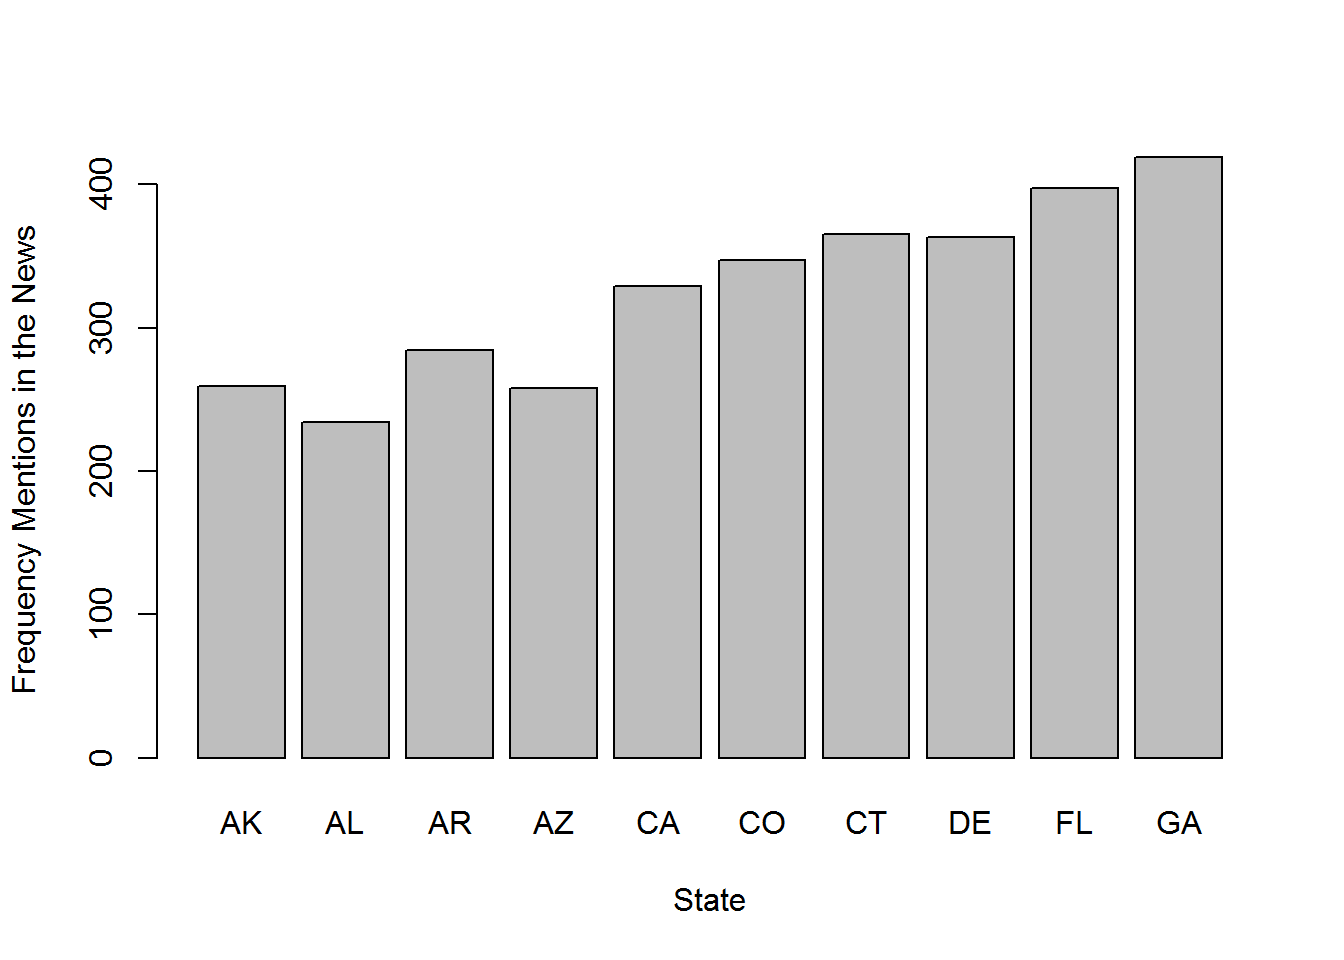
\includegraphics{Multilevel_Models_files/figure-latex/unnamed-chunk-2-1.pdf}

\emph{Figure 1.12.1}

\hypertarget{random-slope-random-intercept}{%
\subsubsection{1.13 Random Slope, Random
Intercept}\label{random-slope-random-intercept}}

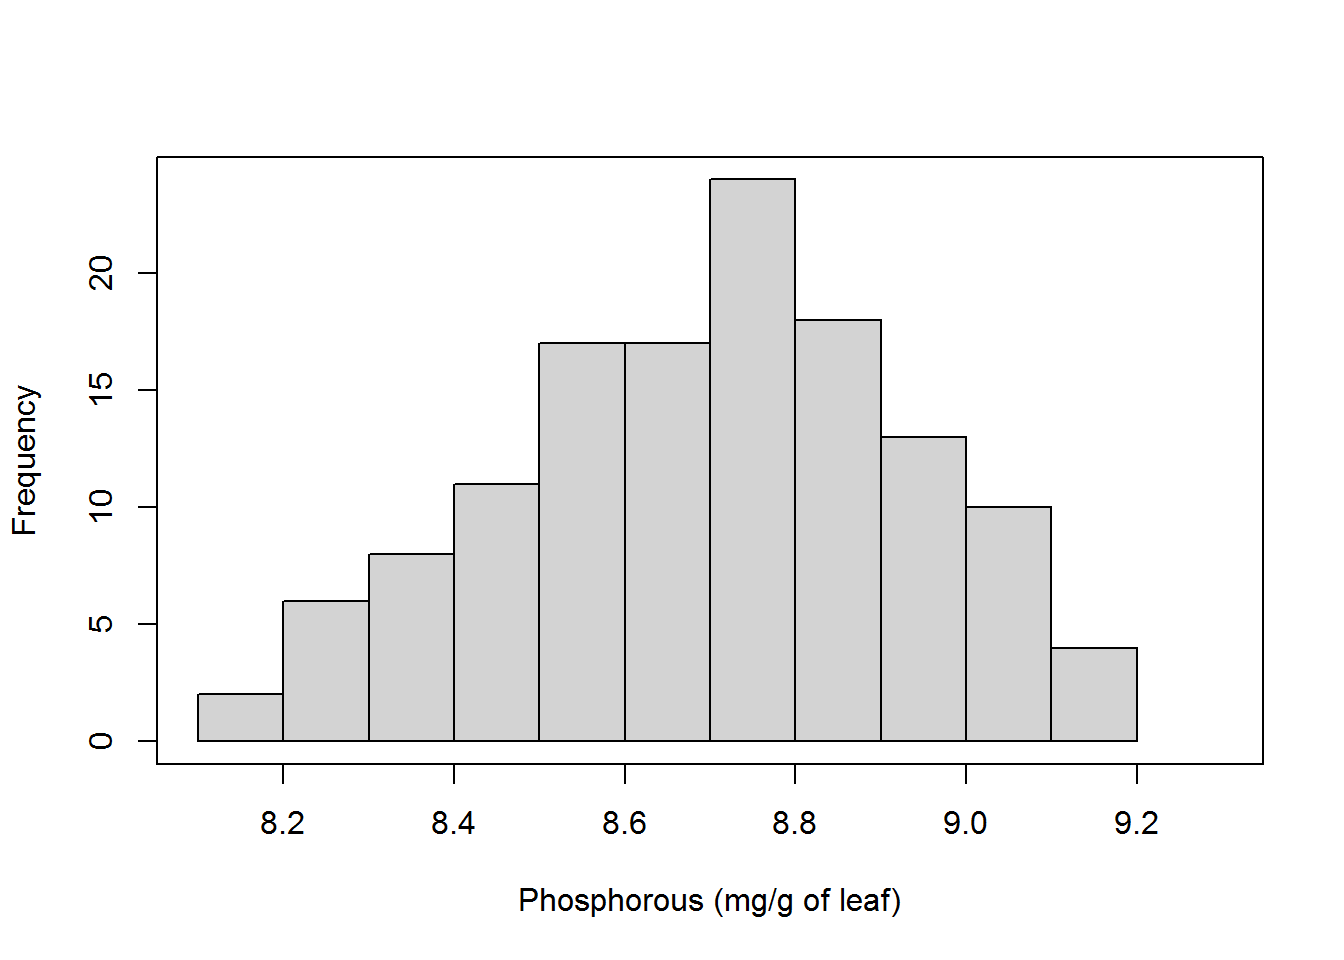
\includegraphics{Multilevel_Models_files/figure-latex/unnamed-chunk-3-1.pdf}

\emph{Figure 1.13.1}

\hypertarget{how-to-represent-these-models}{%
\subsubsection{1.14 How to Represent These
Models}\label{how-to-represent-these-models}}

Fixed intercepts and slopes

QoL after Surgery\textsubscript{i} =\(b_0+b_1Sugery_i+\varepsilon_i\)

Random intercepts and fixed slopes

\(Y_{ij}=b_{0j}+b_1X_{ij}+\varepsilon_{ij}\)

\(b_{0j}=b_0+u_{0j}\)

Fixed intercepts and random slopes

\(Y_{ij}=b_{oi}+b_{1j}X{ij}+\varepsilon{ij}\)

\(b_{1j}=b_1+u_{1j}\)

Random intercepts and random slopes

\(Y_{ij}=b_{oi}+b_{1j}X{ij}+\varepsilon{ij}\)

\(b_{0j}=b_0+u_{0j}\)

\(b_{1j}=b_1+u_{1j}\)

\hypertarget{the-surgery-example}{%
\subsubsection{1.15 The Surgery Example}\label{the-surgery-example}}

Fixed intercepts and slopes

QoL after Surgery\textsubscript{i} =\(b_0+b_1Sugery_i+\varepsilon_i\)

Random intercepts and random slopes

QoL
After\textsubscript{ij}=\(b_{0j}+b_{1j}Surgery_{ij}+b_2QoL \ Before_{ij}+\varepsilon_{ij}\)

\(b_{0j}=b_0+u_{0j}\)

\(b_{0j}=b_0+u_{0j}\)

\hypertarget{comparing-models}{%
\subsubsection{1.16 Comparing Models}\label{comparing-models}}

Models should be built up gradually

\begin{itemize}
\tightlist
\item
  Start with fixed coefficients
\item
  Change one aspect of the model and compare to the previous with the
  change in the -2LL
\end{itemize}

Assessing fit

\begin{itemize}
\tightlist
\item
  AIC
\item
  BIC
\end{itemize}

\hypertarget{covariance-structures}{%
\subsubsection{1.17 Covariance Structures}\label{covariance-structures}}

Variance components

\begin{itemize}
\item
  Random effects are independent with similar variances Diagonal
\item
  Random effects are independent with different variances
\end{itemize}

AR(1)

\begin{itemize}
\tightlist
\item
  Random effects are related with data points closer in time being more
  similar than those distant in time
\item
  Variances of random effects are similar
\end{itemize}

Unstructured

+Covariances and variances of random effects are unpredictable

\hypertarget{centering}{%
\subsubsection{1.18 Centering}\label{centering}}

Grand mean centering

\begin{itemize}
\tightlist
\item
  Take each score and subtract from it the mean of all scores (for that
  variable)
\end{itemize}

Group mean centering

\begin{itemize}
\tightlist
\item
  Take each score and subtract from it the mean of scores from the same
  group (for that variable)
\end{itemize}

Effects of centering in multilevel models

\begin{itemize}
\tightlist
\item
  The effects are complicated
\item
  Models using centred variables tend to be more stable
\item
  It can help with problems of multicollinearity
\end{itemize}

\hypertarget{picturing-the-data}{%
\subsubsection{1.19 Picturing the Data}\label{picturing-the-data}}

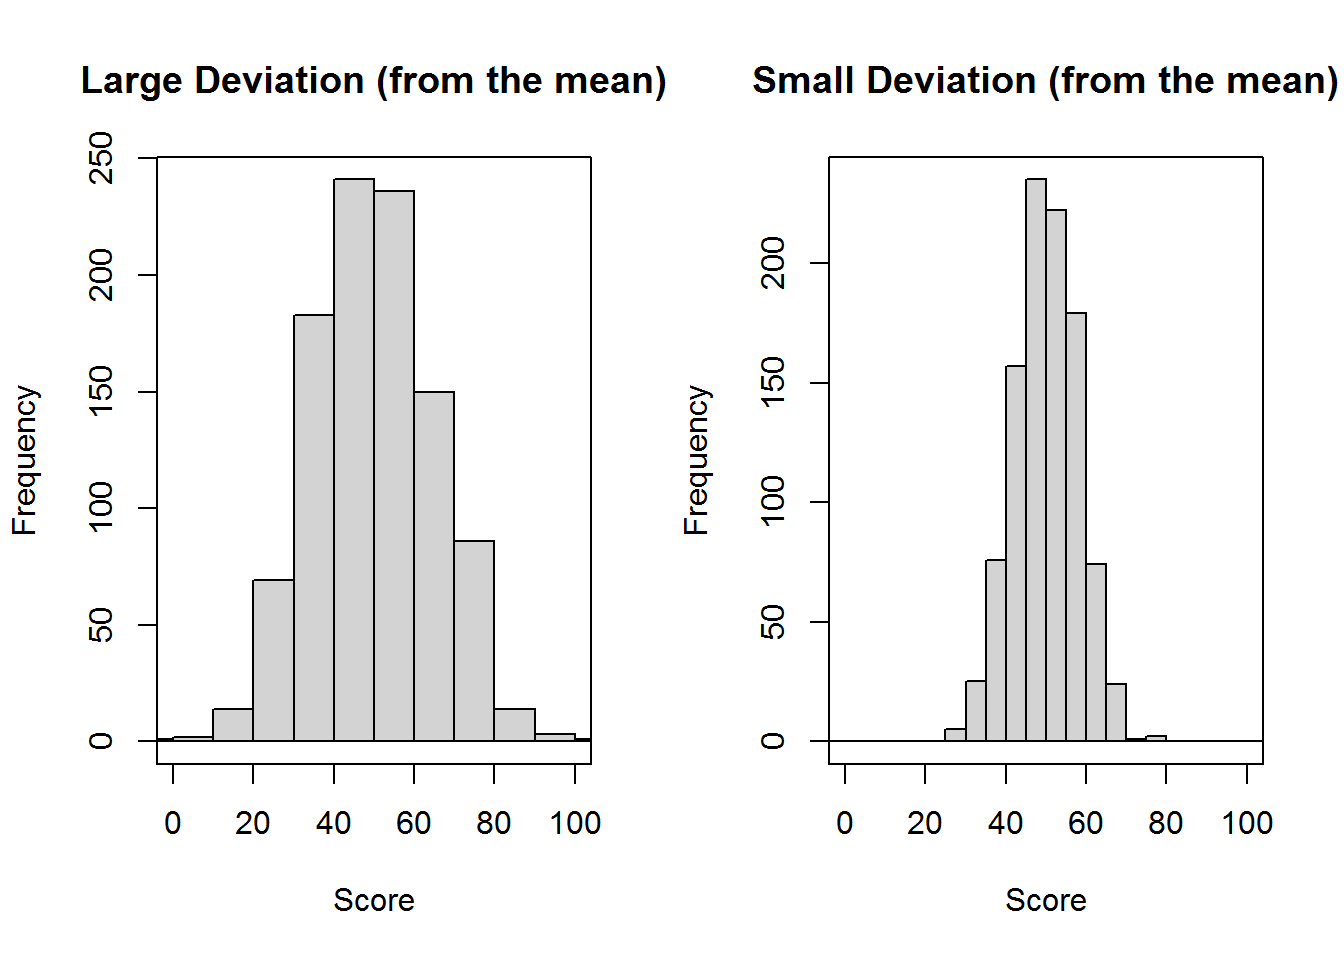
\includegraphics{Multilevel_Models_files/figure-latex/unnamed-chunk-4-1.pdf}

\emph{Figure 1.19.1}

\hypertarget{compare-models}{%
\subsubsection{1.20 Compare Models}\label{compare-models}}

We can have a look at how the fit of the models has improved using the
anova() function that we used before; the following will compare all
three models that we have so far fitted):

\begin{itemize}
\tightlist
\item
  anova(randomInterceptOnly
\item
  randomInterceptSurgery
\item
  randomInterceptSurgeryQoL)
\end{itemize}

\begin{longtable}[]{@{}llllllll@{}}
\toprule
Model & df & AIC & BIC & LogLik & Test & L.Ratio &
p-value\tabularnewline
\midrule
\endhead
1 & 3 & 1911.473 & 1922.334 & -952.7364 & & &\tabularnewline
2 & 4 & 1910.137 & 1924.619 & -951.0686 & 1 vs 2 & 3.33564 &
0.0678\tabularnewline
3 & 5 & 1847.490 & 1865.592 & -918.7450 & 2 vs 3 & 64.64721 &
\textless.0001\tabularnewline
\bottomrule
\end{longtable}

\emph{Table 1.20.1: ~Comparing three models}

\hypertarget{an-example-the-honeymoon-period}{%
\subsubsection{1.21 An Example: The `Honeymoon
Period'}\label{an-example-the-honeymoon-period}}

Speed dating event

\begin{itemize}
\tightlist
\item
  After a speed dating event data were collected on all people who ended
  up in a relationship with the person that they met on the speed dating
  night.
\item
  None of the people measured were in the same relationship.
\end{itemize}

Satisfaction\_Baseline

\begin{itemize}
\tightlist
\item
  A 10-point scale (0 = completely dissatisfied, 10 = completely
  satisfied)
\end{itemize}

Satisfaction\_6\_Months

\begin{itemize}
\tightlist
\item
  Life satisfaction at 6 months (0-10)
\end{itemize}

Satisfaction\_12\_Months

\begin{itemize}
\tightlist
\item
  Life satisfaction at 12 months (0-10)
\end{itemize}

Satisfaction\_18\_Months

\begin{itemize}
\tightlist
\item
  Life satisfaction at 18 months (0-10)
\end{itemize}

Gender

\hypertarget{the-data}{%
\subsubsection{1.22 The Data}\label{the-data}}

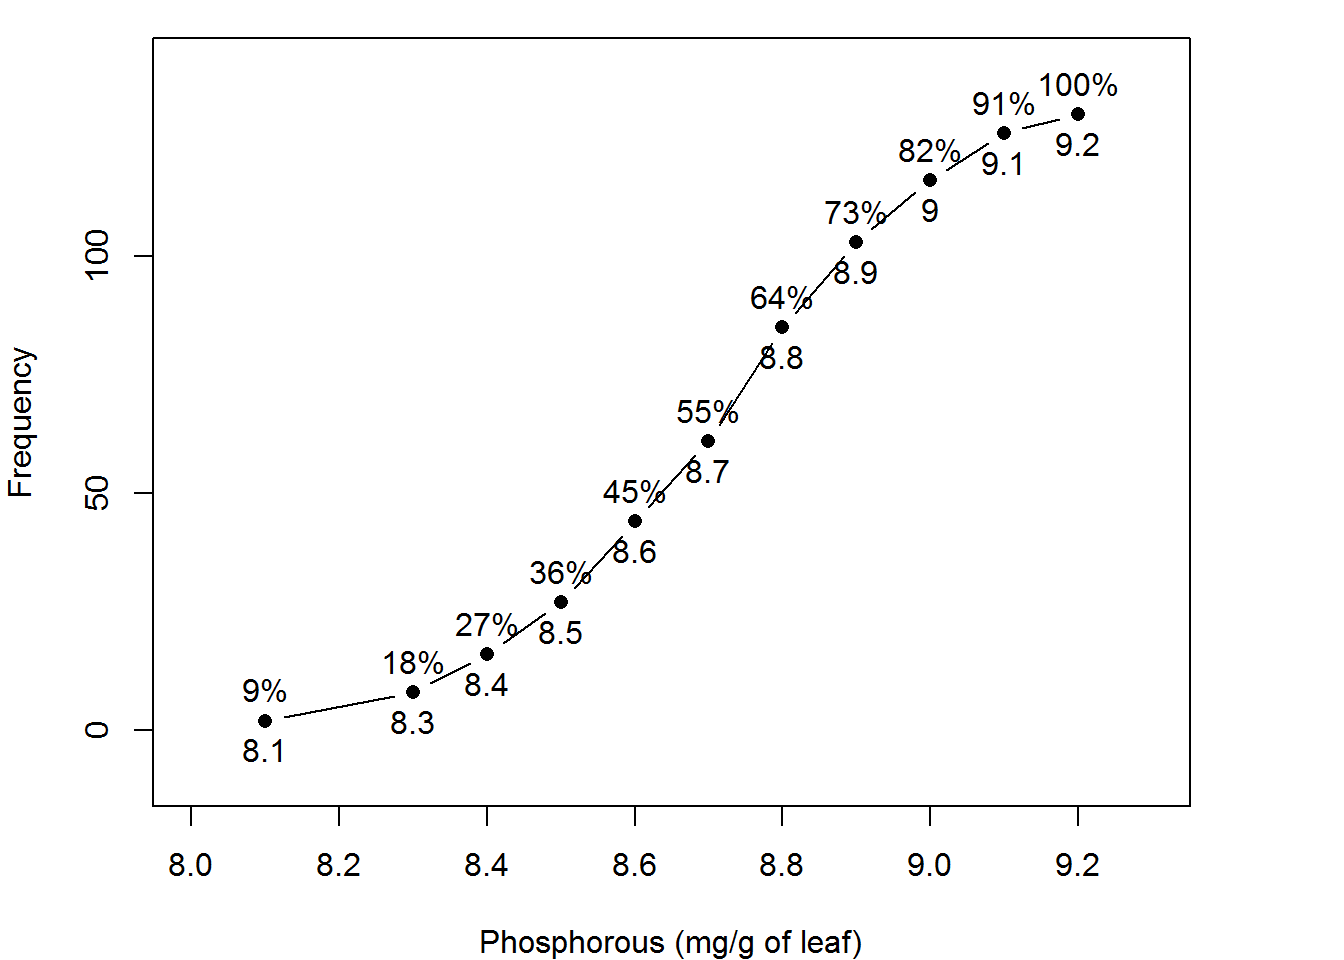
\includegraphics{Multilevel_Models_files/figure-latex/unnamed-chunk-5-1.pdf}

\emph{Figure 1.22.1}

\hypertarget{restructuring-data}{%
\subsubsection{1.23 Restructuring Data}\label{restructuring-data}}

Data entry for multilevel models . Need the variable Time to be
represented by a single column. We refer to this format as the `long'
format. As such we need to restructure the data.

But, in repeated measures designs we're used to entering data so that
instances of the outcome appear in different columns.

\hypertarget{introducing-random-slopes}{%
\subsubsection{1.24 Introducing Random
Slopes}\label{introducing-random-slopes}}

We use the update() function to create a new model (called timeRS) which
is identical to the previous model (timeRI) but updates the random part
of the model to be random = \textasciitilde Time\textbar Person:

\begin{itemize}
\tightlist
\item
  timeRS\textless-update(timeRI, random =
  \textasciitilde Time\textbar Person)
\end{itemize}

\hypertarget{to-sum-up}{%
\subsubsection{1.25 To Sum Up}\label{to-sum-up}}

Data can be hierarchical and this hierarchical structure can be
important.

\begin{itemize}
\tightlist
\item
  Most of the tests that you learn simply ignore the hierarchy.
\end{itemize}

Hierarchical models are just a fancy regression in which you can
estimate the variability in the slopes and intercepts within entities.

\begin{itemize}
\tightlist
\item
  Slopes and intercepts can be random variables (allowed to vary) rather
  than fixed (assumed to be equal in different situations).
\end{itemize}

Start with a model that ignores the hierarchy and then add in random
intercepts and slopes to see if they improve the fit of the model.

Growth curves model trends in the data over time

\begin{itemize}
\tightlist
\item
  These trends can also have variable intercepts and slopes.
\end{itemize}

\end{document}
